\section{Evaluation}

We have written a prototype compiler for \sysname that is implemented in roughly 5000 lines of F\# code. The compiler includes command-line flags for enabling or disabling the use of BGP MED, AS path prepending, the commonly used no-export community, as well as for ensuring k-failure safety for user-sepcified aggregates. The compiler uses regular expressions derivatives~\ref{bib:todo} with character classes to construct automata for large alphabets efficiently. The compiler uses the algorithm for computing graph dominators described in~\ref{bib:todo}. When computing local preferences and failure safety, as described in Section~\ref{sec:compilation}, the compiler performs memoization of the ``can prefer'' relation. \todo{this needs work}

We have evaluated our compiler by translating and compiling real-world network configurations for data centers and a core backbone network into \sysname. We evaluate our compiler by measuring compilation times for these policies across topologies of different sizes.

\begin{figure}[t!]
\centering
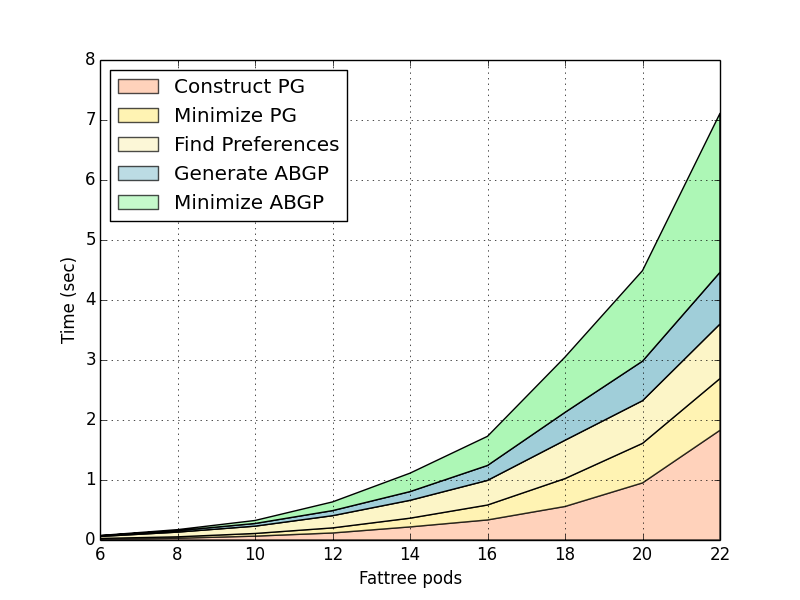
\includegraphics[width=\columnwidth]{figures/compilation-times-dc.png}
\label{fig:compilation-times-dc}
\caption{Data center compilation times.}
\end{figure}

\begin{figure}[t!]
\centering
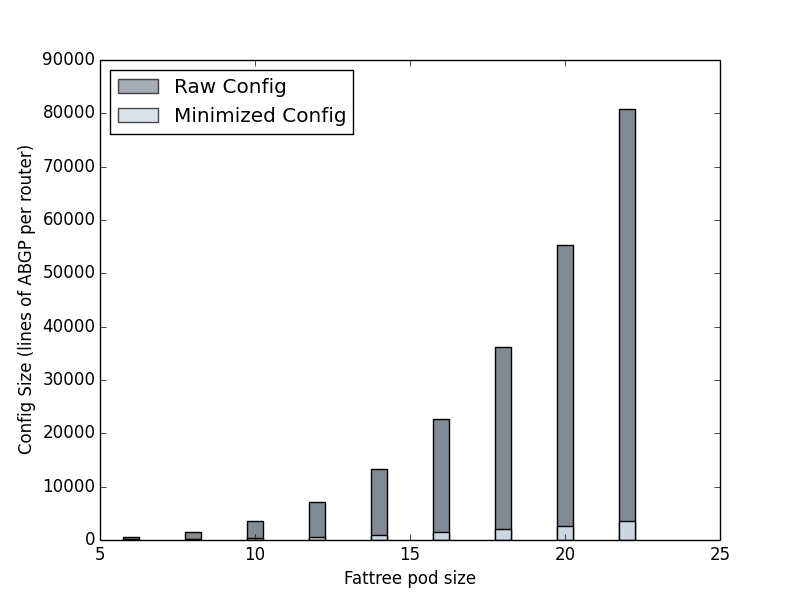
\includegraphics[width=\columnwidth]{figures/config-compression-dc.png}
\label{fig:compilation-compression-dc}
\caption{Data center config minimization.}
\end{figure}